% Based on "Meta-­Activity: Activity Structure" by Clif Kussmaul

\model{The Learning Cycle}

POGIL activities typically form a Learning Cycle, which guides students through three phases, usually with several questions in each phase:

\vspace{1em}

\begin{minipage}{0.68\linewidth}
\begin{itemize}

\item \textbf{Exploration} (E): students collect information and examine data in the model; students answer directly from the information provided or from prior knowledge, without substantial analysis or synthesis.

\item \textbf{Concept Invention / Term Introduction} (I): students find patterns in the data and converge on a concept by answering questions that analyze, compare, and contrast. Terms are introduced after concepts have been developed.

\item \textbf{Application} (A): students test their understanding by applying concepts in new contexts.

\end{itemize}
\end{minipage}
\hfill
\begin{minipage}{0.30\linewidth}
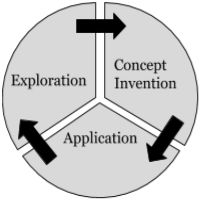
\includegraphics[width=\linewidth]{learning-cycle.png}
\end{minipage}


\quest{15 min}


\Q Go back to ``Activity 6: Recursion'' and label each question with an \textbf{E} for Exploration, an \textbf{I} for Concept Invention / Term Introduction, or an \textbf{A} for Application. (Some questions may be assigned to more than one phase.)

\begin{answer}[1em]
\end{answer}


\Q Does the activity generally follow the Learning Cycle? Why or why not?

\begin{answer}
\end{answer}


\Q What are the pros and cons of having Concept Invention precede Term Introduction?

\begin{answer}
\end{answer}


\Q What is the value of including open-­ended questions in a POGIL activity?

\begin{answer}
\end{answer}
